\section{Reachi Experiments}\label{sec:linkmodel}
\todo[inline]{introduce the data. WIP}
To verify that our model for computing path loss gives proper results, we have received data from conducted experiments from the Reachi project.

\todo[inline]{talk about the problems with the data. WIP}
When we detected odd behaviour, we started to investigate the logs. Specifically the logs from experiments
conducted in Marikina and Rude Skov. The reason for these two, is that the Rude Skov log was not conducted in
the middle of a city while the Marikina was, as such the Marikina log should contain more varying signal
strength measurements because there is more dense obstructions that can influence the signal. We used the
distance dependent fading function from \cite{paper:linkmodel}, that computes path loss based on the distance
of a link, where we compared the measurements with transmission power - path loss computed from the distance
fading function.

On plot \ref{plot:reachi-experiments:average-distance} the measurements and distance fading function RSSI
values can be seen. The measurements have been divided into distance buckets, where the average for each
bucket has been computed and plotted.

\begin{figure}[H]
    \centering
    \begin{tikzpicture}%\label{plot:reachi-experiments:average-distance}
        \begin{axis}[
                height=12cm, width=0.95\textwidth,
                ylabel={RSSI},
                xlabel={Distance in meters},
                axis lines*=left,
                xmin=0, xmax=750,
                enlargelimits=false,
                ymin=-120, ymax=-20,
                xtick={0, 50, 100, 150, 200, 250, 300, 350, 400, 450, 500, 550, 600, 650, 700, 750},
                ymajorgrids=true,
                xmajorgrids=true,
                grid style=dashed,
                restrict y to domain=-120:-20,
                samples=600
            ]

            \addplot[very thick, solid, cyan, mark=*] coordinates {(20, -28.32345013477089) (40, -44.85830258302583) (60, -52.77323717948718) (80, -60.21201657458563) (100, -66.47435897435898) (120, -69.68905472636816) (140, -71.5976496922216) (160, -73.7866473149492) (180, -75.53428571428572) (200, -76.89289392378991) (220, -77.88135593220339) (240, -77.8035019455253) (260, -77.36784140969164) (280, -77.14030612244898) (300, -77.75299760191847) (320, -79.71686746987952) (340, -79.15481171548117) (360, -79.90728476821192) (380, -81.30909090909091) (400, -81.79746835443038) (420, -81.52272727272727) (440, -79.2) (460, -79.42105263157895) (480, -79.4375) (500, -79.0) (520, -77.91666666666667) (540, -83.0) (560, -81.27272727272727) (580, -83.57142857142857) (600, -86.0) (620, -83.4) (640, -86.5) (660, -81.42857142857143) (680, -79.0) (700, -82.71428571428571) (740, -77.0)};
            \addlegendentry{Marikina field measurements};


            \addplot[domain=0:740, very thick, solid, red] {26 - ld(x)};
            \addlegendentry{distance path loss function};
        \end{axis}
    \end{tikzpicture}
    \caption{Average RSSI pr. distance}\label{plot:reachi-experiments:average-distance}
\end{figure}







\newpage
\section{Line of Sight Model (LoSModel)}
\todo[inline]{ref to section where field experiments problems discussed}
To facilitate the problems mentioned in \autoref{sec:reachi-data-experiments}, we have developed our own model for computing path loss. The model, called \gls{losmodel}, computes path loss based on the distance of the link and the percentage of the link that contains building as an obstruction. The idea is that large obstructions, like buildings, cause more severe loss of signal strength compared to a purely distance based approach. Our model only considers buildings as an obstruction, and is therefore to be taking as a proof of concept. \autoref{algo:losmodel:computepathloss} is a pseudo code implementation of the path loss computation.



\subsection{\acrfull{cvpl} and \acrfull{bopl}}
To compute the path loss of a link with buildings having more severe impact, we define the functions \gls{cvpl} and \gls{bopl}.
% \begin{eq*}%\label{eq:losmodel:cvpl}
%     \mathit{cvpl}(l) = (48.5 * (\ln(d(l)) / \ln(77)) + 37.5);
% \end{eq*}

% \begin{eq*}\label{eq:losmodel:bopl}
%     \mathit{bopl}(l) = (67 * (\ln(d(l)) / \ln(57)) + 11.5);
% \end{eq*}

Both functions compute path loss based on distance. \gls{cvpl} computes path loss for distances with zero percent building, while \gls{bopl} computes path loss for 100\% building. Samples drawn from both functions have been plotted on \autoref{plot:reachi-experiments:cvpl-vs-bopl}. From looking at \autoref{plot:reachi-experiments:cvpl-vs-bopl} \gls{bopl} causes a more severe path loss compared to \gls{cvpl}.\medbreak

To find the constants for both functions, data for comparison is needed. Links with a computed building percentage below five percent or above 80\% was collected from the Marikina log into their separate collections. The Marikina log was used because the experiment was conducted in a city, resulting in links with varying building percentages.

For both collections the links was further separated based on distance of the links, with 20 meter intervals i.e. links with distance between 20 meters and 40 meters was separated together. The average \gls{rssi} for each separation was then computed and now ready to be used as comparison data. To approximate the constants for both functions, brute forcing was used on the following function:
\begin{eq}
    \alpha \cdot (\ln{x} / \ln{\delta}) + \beta
\end{eq}

$x$ is the distance, $\alpha,\ \beta \in \{-100,\dots, 100\}$ with $0.5$ increments and $\delta \in \{2, 100\}$ with increments of $1$. The samples drawn will then be compared with the computed samples \textbf{before} with the following score function:
\begin{eq}
    \mathlarger{compare(l_1, l_2) =|(l_1.rssi - l_d(d(l_1))) - (l_2.rssi - pl(d(l_2)))|}
\end{eq}

\begin{eq}
    score(l_1, l_2) = \mathlarger{\sum}\limits_{l_1,\ l_2\ \in\ links} (compare(l_1, l_2))^2
\end{eq}

The result gives the following functions:
%\begin{eq}
%    cvpl(l) = 48.5 \cdot (\ln{(d(l)) / \ln{(77)}) + 37.5
%\end{eq}
%
%\begin{eq}
%    bopl(l) = 67 \cdot (\ln{(d(l))} / \ln{(57)) + 11.5
%\end{eq}



\begin{figure}[H]
    \centering
    \begin{tikzpicture}
        \begin{axis}[
                height=12cm, width=0.95\textwidth,
                ylabel={RSSI},
                xlabel={Distance in meters},
                axis lines*=left,
                xmin=0, xmax=750,
                enlargelimits=false,
                ymajorgrids=true,
                xmajorgrids=true,
                grid style=dashed,
                restrict y to domain=-120:0,
                samples=700
            ]

            \addplot[domain=0:1000, very thick, solid, cyan] {26 - bopl(x)};
            \addlegendentry{\gls{bopl}};

            \addplot[domain=0:1000, very thick, solid, red] {26 - cvpl(x)};
            \addlegendentry{\gls{cvpl}};
        \end{axis}
    \end{tikzpicture}
    \caption{Plot showing sampels drawn from \gls{cvpl} and \gls{bopl}}
    \label{plot:reachi-experiments:cvpl-vs-bopl}
\end{figure}


\begin{figure}[H]
    \centering
    \begin{tikzpicture}%\label{plot:reachi-experiments:average-distance}
        \begin{axis}[
                title=score - 501.586,
                height=12cm, width=0.95\textwidth,
                ylabel={RSSI},
                xlabel={Distance in meters},
                axis lines*=left,
                xmin=0, xmax=750,
                enlargelimits=false,
                ymin=-90, ymax=-30,
                xtick={0, 50, 100, 150, 200, 250, 300, 350, 400, 450, 500, 550, 600, 650, 700, 750},
                ymajorgrids=true,
                xmajorgrids=true,
                grid style=dashed,
                samples=700
            ]

            \addplot[very thick, solid, cyan, mark=*] coordinates {(20, -36.01344537815126) (40, -48.361111111111114) (60, -54.93279022403259) (80, -62.40816326530612) (100, -68.14871794871794) (120, -60.85954712362301) (140, -71.69568452380952) (160, -74.36896551724138) (180, -73.93817204301075) (200, -75.09929078014184) (220, -73.38403041825094) (240, -75.43994413407822) (260, -77.69102990033223) (280, -77.31512605042016) (300, -75.7751937984496) (320, -78.60714285714286) (340, -78.38524590163935) (360, -78.52459016393442) (380, -77.34285714285714) (400, -80.96153846153847) (420, -81.03571428571429) (440, -80.41379310344827) (460, -74.18181818181819) (480, -79.9090909090909) (500, -79.75) (520, -77.56521739130434) (540, -81.23076923076923) (560, -78.9) (580, -85.0) (620, -82.5) (640, -82.33333333333333) (660, -82.4) (680, -77.5) (700, -85.4) (740, -77.0)};
            \addlegendentry{Marikina field measurements}


            \addplot[domain=0:740, very thick, solid, red] {26 - cvpl(x)};
            \addlegendentry{\gls{cvpl}};


        \end{axis}
    \end{tikzpicture}
    \caption{Field measurements with building percentage below 5\%}
    \label{plot:reachi-experiments:marikina-log-below-5-pct}
\end{figure}



\begin{figure}[H]
    \centering
    \begin{tikzpicture}%\label{plot:reachi-experiments:average-distance}
        \begin{axis}[
                title=score - 350.722,
                height=12cm, width=0.95\textwidth,
                ylabel={RSSI},
                xlabel={Distance in meters},
                axis lines*=left,
                xmin=0, xmax=380,
                enlargelimits=false,
                ymin=-90, ymax=-30,
                ymajorgrids=true,
                xmajorgrids=true,
                grid style=dashed,
                samples=400
            ]

            \addplot[very thick, solid, cyan, mark=*] coordinates {(20, -32.56521739130435) (40, -50.607142857142854) (60, -52.15384615384615) (80, -64.85714285714286) (100, -49.5) (120, -65.76623376623377) (140, -69.38888888888889) (160, -72.05714285714286) (180, -69.3125) (200, -78.83333333333333) (220, -76.84) (240, -75.75) (260, -80.91666666666667) (280, -72.88888888888889) (300, -78.95238095238095) (320, -76.44444444444444) (340, -82.75) (380, -87.0)};
            \addlegendentry{Marikina field measurements};

            \addplot[domain=0:380, very thick, solid, red] {26 - bopl(x)};
            \addlegendentry{\gls{bopl}};


        \end{axis}
    \end{tikzpicture}
    \caption{Field measurements with building percentage above 80\%}
    \label{plot:reachi-experiments:marikina-log-above-80-pct}
\end{figure}





\begin{algorithm}[H]
    \DontPrintSemicolon
    \SetKwFunction{FLoSModelCompute}{ComputePathloss}
    \SetKwProg{Fn}{Function}{}{}

    $\mathit{map} \leftarrow$ A map of an area\;
    \;
    \Fn{\FLoSModelCompute{$l$}}{
        $n_1, n_2 \leftarrow \mathit{nodes}(l)$\;
        $p_1 \leftarrow$ compute pixel position on $\mathit{map}$ for $n_1$\;
        $p_2 \leftarrow$ compute pixel position on $\mathit{map}$ for $n_2$\;
        $\mathit{bearing} \leftarrow$ compute bearing between $p_1$ and $p_2$\;
        $\mathit{pixels} \leftarrow 0$\;
        $\mathit{buildings} \leftarrow 0$\;
        $x \leftarrow p_{2,x}$\;
        $y \leftarrow p_{2,y}$\;
        \;
        \While{$x \geq p_{1,x}$ \KwAnd $y \geq p_{1,y}$}{
            $\mathit{colour} \leftarrow$ get colour of $(x, y)$ on $\mathit{map}$\;
            \If{$\mathit{colour}$ \KwIs building}{
                $\mathit{buildings} \leftarrow \mathit{buildings} + 1$\;
            }
            $x \leftarrow x - 1$\;
            $y \leftarrow y - \mathit{bearing}$\;
            $\mathit{pixels} \leftarrow \mathit{pixels} + 1$\;
        }
        \;
        $\mathit{pct} \leftarrow \mathit{buildings} / \mathit{pixels}$\;
        $\mathit{pl}_l \leftarrow (\mathit{cvpl}(l) \cdot 1 - pct) + (\mathit{bopl}(l) \cdot pct)$\;

        \KwRet $\mathit{pl_l}$\;
    }
    \caption{The ComputePathloss function.}
    \label{algo:losmodel:computepathloss}
\end{algorithm}

\bigbreak


In \autoref{plot:reachi-experiments:marikina-log-above-80-pct} and \autoref{plot:reachi-experiments:marikina-log-below-5-pct}.





\begin{figure}[H]
    \centering
    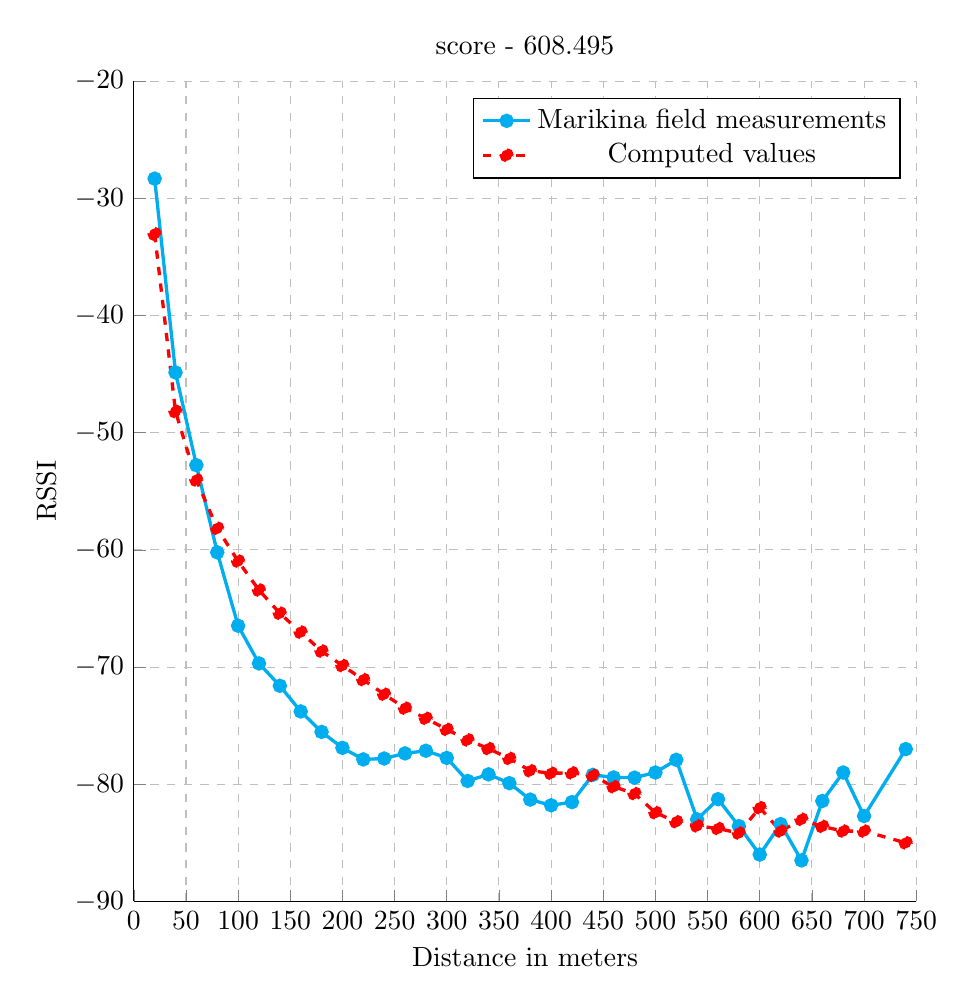
\begin{tikzpicture}%\label{plot:reachi-experiments:average-distance}
        \begin{axis}[
                title=score - 608.495,
                height=12cm, width=0.95\textwidth,
                ylabel={RSSI},
                xlabel={Distance in meters},
                axis lines*=left,
                xmin=0, xmax=750,
                enlargelimits=false,
                ymin=-90, ymax=-20,
                xtick={0, 50, 100, 150, 200, 250, 300, 350, 400, 450, 500, 550, 600, 650, 700, 750},
                ymajorgrids=true,
                xmajorgrids=true,
                grid style=dashed,
            ]

            \addplot[very thick, solid, cyan, mark=*] coordinates {(20, -28.32345013477089) (40, -44.85830258302583) (60, -52.77323717948718) (80, -60.21201657458563) (100, -66.47435897435898) (120, -69.68905472636816) (140, -71.5976496922216) (160, -73.7866473149492) (180, -75.53428571428572) (200, -76.89289392378991) (220, -77.88135593220339) (240, -77.8035019455253) (260, -77.36784140969164) (280, -77.14030612244898) (300, -77.75299760191847) (320, -79.71686746987952) (340, -79.15481171548117) (360, -79.90728476821192) (380, -81.30909090909091) (400, -81.79746835443038) (420, -81.52272727272727) (440, -79.2) (460, -79.42105263157895) (480, -79.4375) (500, -79.0) (520, -77.91666666666667) (540, -83.0) (560, -81.27272727272727) (580, -83.57142857142857) (600, -86.0) (620, -83.4) (640, -86.5) (660, -81.42857142857143) (680, -79.0) (700, -82.71428571428571) (740, -77.0)};
            \addlegendentry{Marikina field measurements};

            \addplot[very thick, dashed, red, mark=*] coordinates {(20,-33.04359925788497)(40,-48.19327731092437)(60,-54.03703703703704)(80,-58.16688567674113)(100,-60.96085858585859)(120,-63.43184421534937)(140,-65.41129831516353)(160,-67.02463054187191)(180,-68.64031007751937)(200,-69.87730061349693)(220,-71.07770961145194)(240,-72.32267441860465)(260,-73.50986842105263)(280,-74.37786259541984)(300,-75.32413793103449)(320,-76.22083333333333)(340,-76.95930232558139)(360,-77.8018018018018)(380,-78.84883720930233)(400,-79.06557377049181)(420,-79.03030303030303)(440,-79.25)(460,-80.21428571428571)(480,-80.8)(500,-82.42857142857143)(520,-83.2)(540,-83.55555555555556)(560,-83.77777777777777)(580,-84.16666666666667)(600,-82.0)(620,-84.0)(640,-83.0)(660,-83.6)(680,-84.0)(700,-84.0)(740,-85.0)};
            \addlegendentry{Computed values};
        \end{axis}
    \end{tikzpicture}
    \caption{Field measurements vs computed values}
    \label{plot:reachi-experiments:phili-log-vs-computed}
\end{figure}


\begin{figure}[H]
    \centering
    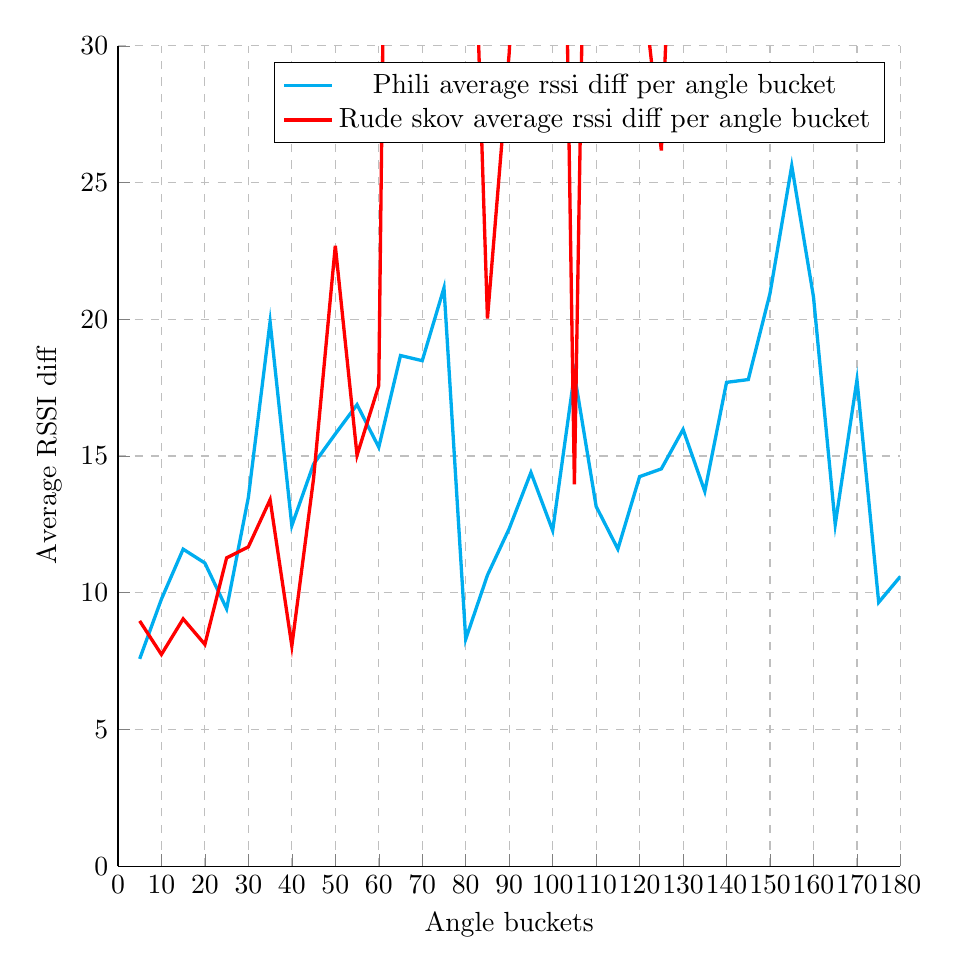
\begin{tikzpicture}%\label{plot:reachi-experiments:average-distance}
        \begin{axis}[
                height=12cm, width=0.95\textwidth,
                ylabel={Average RSSI diff},
                xlabel={Angle buckets},
                axis lines*=left,
                xmin=0, xmax=180,
                xtick={0, 10, 20, 30, 40, 50, 60, 70, 80, 90, 100, 110, 120, 130, 140, 150, 160,170,180},
                enlargelimits=false,
                ymin=0, ymax=30,
                ymajorgrids=true,
                xmajorgrids=true,
                grid style=dashed
            ]

            %\addplot[very thick, solid, cyan!50!black] coordinates {(5, 7.581215097994852) (10, 9.763581254686114) (15, 11.59234807189617) (20, 11.084399582147876) (25, 9.411670936293284) (30, 13.486232393853125) (35, 19.91110051641767) (40, 12.453590557884946) (45, 14.70313120243339) (50, 15.804939314638208) (55, 16.87697870999425) (60, 15.320902904198922) (65, 18.673392004683087) (70, 18.48508963612783) (75, 21.147550183881993) (80, 8.302184073487094) (85, 10.641508684206432) (90, 12.343183048128944) (95, 14.396643466792797) (100, 12.27504884861337) (105, 17.994872329043496) (110, 13.156645245862158) (115, 11.595967499573286) (120, 14.245146945189493) (125, 14.528392002600814) (130, 15.96981736460891) (135, 13.70427190114752) (140, 17.692009757218077) (145, 17.79486440192431) (150, 20.947579654378668) (155, 25.611175147469265) (160, 20.819124899373364) (165, 12.495568407794714) (170, 17.784042978338544) (175, 9.646875797269503) (180, 10.597197732034614)};
            \addplot[very thick, solid, cyan] coordinates {(5,7.581215097994852)(10,9.763581254686114)(15,11.59234807189617)(20,11.084399582147876)(25,9.411670936293284)(30,13.486232393853125)(35,19.91110051641767)(40,12.453590557884946)(45,14.70313120243339)(50,15.804939314638208)(55,16.87697870999425)(60,15.320902904198922)(65,18.673392004683087)(70,18.48508963612783)(75,21.147550183881993)(80,8.302184073487094)(85,10.641508684206432)(90,12.343183048128944)(95,14.396643466792797)(100,12.27504884861337)(105,17.994872329043496)(110,13.156645245862158)(115,11.595967499573286)(120,14.245146945189493)(125,14.528392002600814)(130,15.96981736460891)(135,13.70427190114752)(140,17.692009757218077)(145,17.79486440192431)(150,20.947579654378668)(155,25.611175147469265)(160,20.819124899373364)(165,12.495568407794714)(170,17.784042978338544)(175,9.646875797269503)(180,10.597197732034614)};
            \addlegendentry{Phili average rssi diff per angle bucket};


            %\addplot[very thick, solid, red!50!black] coordinates {(5, 8.968175725354994) (10, 7.741408675352775) (15, 9.042742837449076) (20, 8.108954051047618) (25, 11.273321343260399) (30, 11.67692967914715) (35, 13.401460743255232) (40, 8.053793318539391) (45, 14.17474549040368) (50, 22.68855220716477) (55, 15.026896145186285) (60, 17.5755161176863) (65, 85.01233086400362) (70, 59.69038212814202) (75, 62.41948703096457) (80, 44.72712810089782) (85, 20.029080610052482) (90, (29.737954905927445) (95, 43.39235466255519) (100, 64.720015835849) (105, 13.965589072181558) (110, 61.334883149884675) (115, 36.30455538419785) (120, 33.32223486902817) (125, 26.172354285886417) (130, 45.62355888699502) (135, 55.8474401182669) (140, 47.511612928722954) (145, 49.70429537245245) (150, 50.649080550831435) (155, 52.34402139529124) (160, 51.45218633523966) (165, 51.805898996936115) (170, 52.39131328924595) (175, 48.78102582759046) (180, 51.91529108595685)};
            \addplot[very thick, solid, red] coordinates {(5,8.968175725354994)(10,7.741408675352775)(15,9.042742837449076)(20,8.108954051047618)(25,11.273321343260399)(30,11.67692967914715)(35,13.401460743255232)(40,8.053793318539391)(45,14.17474549040368)(50,22.68855220716477)(55,15.026896145186285)(60,17.5755161176863)(65,85.01233086400362)(70,59.69038212814202)(75,62.41948703096457)(80,44.72712810089782)(85,20.029080610052482)(90,29.737954905927445)(95,43.39235466255519)(100,64.720015835849)(105,13.965589072181558)(110,61.334883149884675)(115,36.30455538419785)(120,33.32223486902817)(125,26.172354285886417)(130,45.62355888699502)(135,55.8474401182669)(140,47.511612928722954)(145,49.70429537245245)(150,50.649080550831435)(155,52.34402139529124)(160,51.45218633523966)(165,51.805898996936115)(170,52.39131328924595)(175,48.78102582759046)(180,51.91529108595685)};
            \addlegendentry{Rude skov average rssi diff per angle bucket};
        \end{axis}
    \end{tikzpicture}
    \caption{}
    \label{plot:reachi-experiments:avg-rssi-angle-phili-rude}
\end{figure}



\todo[inline]{show some plots, proving the problems}
\todo[inline]{talk about the visualiser + youtube link that shows the problems}
\todo[inline]{shortly mention CVPL and BOPL model that will be introduced in detail later}